% Options for packages loaded elsewhere
\PassOptionsToPackage{unicode}{hyperref}
\PassOptionsToPackage{hyphens}{url}
%
\documentclass[
]{article}
\usepackage{amsmath,amssymb}
\usepackage{iftex}
\ifPDFTeX
  \usepackage[T1]{fontenc}
  \usepackage[utf8]{inputenc}
  \usepackage{textcomp} % provide euro and other symbols
\else % if luatex or xetex
  \usepackage{unicode-math} % this also loads fontspec
  \defaultfontfeatures{Scale=MatchLowercase}
  \defaultfontfeatures[\rmfamily]{Ligatures=TeX,Scale=1}
\fi
\usepackage{lmodern}
\ifPDFTeX\else
  % xetex/luatex font selection
\fi
% Use upquote if available, for straight quotes in verbatim environments
\IfFileExists{upquote.sty}{\usepackage{upquote}}{}
\IfFileExists{microtype.sty}{% use microtype if available
  \usepackage[]{microtype}
  \UseMicrotypeSet[protrusion]{basicmath} % disable protrusion for tt fonts
}{}
\makeatletter
\@ifundefined{KOMAClassName}{% if non-KOMA class
  \IfFileExists{parskip.sty}{%
    \usepackage{parskip}
  }{% else
    \setlength{\parindent}{0pt}
    \setlength{\parskip}{6pt plus 2pt minus 1pt}}
}{% if KOMA class
  \KOMAoptions{parskip=half}}
\makeatother
\usepackage{xcolor}
\usepackage[margin=1in]{geometry}
\usepackage{color}
\usepackage{fancyvrb}
\newcommand{\VerbBar}{|}
\newcommand{\VERB}{\Verb[commandchars=\\\{\}]}
\DefineVerbatimEnvironment{Highlighting}{Verbatim}{commandchars=\\\{\}}
% Add ',fontsize=\small' for more characters per line
\usepackage{framed}
\definecolor{shadecolor}{RGB}{248,248,248}
\newenvironment{Shaded}{\begin{snugshade}}{\end{snugshade}}
\newcommand{\AlertTok}[1]{\textcolor[rgb]{0.94,0.16,0.16}{#1}}
\newcommand{\AnnotationTok}[1]{\textcolor[rgb]{0.56,0.35,0.01}{\textbf{\textit{#1}}}}
\newcommand{\AttributeTok}[1]{\textcolor[rgb]{0.13,0.29,0.53}{#1}}
\newcommand{\BaseNTok}[1]{\textcolor[rgb]{0.00,0.00,0.81}{#1}}
\newcommand{\BuiltInTok}[1]{#1}
\newcommand{\CharTok}[1]{\textcolor[rgb]{0.31,0.60,0.02}{#1}}
\newcommand{\CommentTok}[1]{\textcolor[rgb]{0.56,0.35,0.01}{\textit{#1}}}
\newcommand{\CommentVarTok}[1]{\textcolor[rgb]{0.56,0.35,0.01}{\textbf{\textit{#1}}}}
\newcommand{\ConstantTok}[1]{\textcolor[rgb]{0.56,0.35,0.01}{#1}}
\newcommand{\ControlFlowTok}[1]{\textcolor[rgb]{0.13,0.29,0.53}{\textbf{#1}}}
\newcommand{\DataTypeTok}[1]{\textcolor[rgb]{0.13,0.29,0.53}{#1}}
\newcommand{\DecValTok}[1]{\textcolor[rgb]{0.00,0.00,0.81}{#1}}
\newcommand{\DocumentationTok}[1]{\textcolor[rgb]{0.56,0.35,0.01}{\textbf{\textit{#1}}}}
\newcommand{\ErrorTok}[1]{\textcolor[rgb]{0.64,0.00,0.00}{\textbf{#1}}}
\newcommand{\ExtensionTok}[1]{#1}
\newcommand{\FloatTok}[1]{\textcolor[rgb]{0.00,0.00,0.81}{#1}}
\newcommand{\FunctionTok}[1]{\textcolor[rgb]{0.13,0.29,0.53}{\textbf{#1}}}
\newcommand{\ImportTok}[1]{#1}
\newcommand{\InformationTok}[1]{\textcolor[rgb]{0.56,0.35,0.01}{\textbf{\textit{#1}}}}
\newcommand{\KeywordTok}[1]{\textcolor[rgb]{0.13,0.29,0.53}{\textbf{#1}}}
\newcommand{\NormalTok}[1]{#1}
\newcommand{\OperatorTok}[1]{\textcolor[rgb]{0.81,0.36,0.00}{\textbf{#1}}}
\newcommand{\OtherTok}[1]{\textcolor[rgb]{0.56,0.35,0.01}{#1}}
\newcommand{\PreprocessorTok}[1]{\textcolor[rgb]{0.56,0.35,0.01}{\textit{#1}}}
\newcommand{\RegionMarkerTok}[1]{#1}
\newcommand{\SpecialCharTok}[1]{\textcolor[rgb]{0.81,0.36,0.00}{\textbf{#1}}}
\newcommand{\SpecialStringTok}[1]{\textcolor[rgb]{0.31,0.60,0.02}{#1}}
\newcommand{\StringTok}[1]{\textcolor[rgb]{0.31,0.60,0.02}{#1}}
\newcommand{\VariableTok}[1]{\textcolor[rgb]{0.00,0.00,0.00}{#1}}
\newcommand{\VerbatimStringTok}[1]{\textcolor[rgb]{0.31,0.60,0.02}{#1}}
\newcommand{\WarningTok}[1]{\textcolor[rgb]{0.56,0.35,0.01}{\textbf{\textit{#1}}}}
\usepackage{graphicx}
\makeatletter
\newsavebox\pandoc@box
\newcommand*\pandocbounded[1]{% scales image to fit in text height/width
  \sbox\pandoc@box{#1}%
  \Gscale@div\@tempa{\textheight}{\dimexpr\ht\pandoc@box+\dp\pandoc@box\relax}%
  \Gscale@div\@tempb{\linewidth}{\wd\pandoc@box}%
  \ifdim\@tempb\p@<\@tempa\p@\let\@tempa\@tempb\fi% select the smaller of both
  \ifdim\@tempa\p@<\p@\scalebox{\@tempa}{\usebox\pandoc@box}%
  \else\usebox{\pandoc@box}%
  \fi%
}
% Set default figure placement to htbp
\def\fps@figure{htbp}
\makeatother
\setlength{\emergencystretch}{3em} % prevent overfull lines
\providecommand{\tightlist}{%
  \setlength{\itemsep}{0pt}\setlength{\parskip}{0pt}}
\setcounter{secnumdepth}{-\maxdimen} % remove section numbering
\usepackage{ctex}
\usepackage{bookmark}
\IfFileExists{xurl.sty}{\usepackage{xurl}}{} % add URL line breaks if available
\urlstyle{same}
\hypersetup{
  pdftitle={homework5},
  pdfauthor={zza},
  hidelinks,
  pdfcreator={LaTeX via pandoc}}

\title{homework5}
\author{zza}
\date{2025-07-01}

\begin{document}
\maketitle

\subsection{1}\label{section}

\begin{Shaded}
\begin{Highlighting}[]
\NormalTok{percentile\_ratio\_discrepancies }\OtherTok{\textless{}{-}} \ControlFlowTok{function}\NormalTok{(P99, P99}\FloatTok{.5}\NormalTok{, P99}\FloatTok{.9}\NormalTok{, a) \{}
  
\NormalTok{  term1 }\OtherTok{\textless{}{-}}\NormalTok{ ((P99 }\SpecialCharTok{/}\NormalTok{ P99}\FloatTok{.9}\NormalTok{)}\SpecialCharTok{\^{}}\NormalTok{(}\SpecialCharTok{{-}}\NormalTok{a }\SpecialCharTok{+} \DecValTok{1}\NormalTok{) }\SpecialCharTok{{-}} \DecValTok{10}\NormalTok{)}\SpecialCharTok{\^{}}\DecValTok{2}
\NormalTok{  term2 }\OtherTok{\textless{}{-}}\NormalTok{ ((P99}\FloatTok{.5} \SpecialCharTok{/}\NormalTok{ P99}\FloatTok{.9}\NormalTok{)}\SpecialCharTok{\^{}}\NormalTok{(}\SpecialCharTok{{-}}\NormalTok{a }\SpecialCharTok{+} \DecValTok{1}\NormalTok{) }\SpecialCharTok{{-}} \DecValTok{5}\NormalTok{)}\SpecialCharTok{\^{}}\DecValTok{2}
\NormalTok{  term3 }\OtherTok{\textless{}{-}}\NormalTok{ ((P99 }\SpecialCharTok{/}\NormalTok{ P99}\FloatTok{.5}\NormalTok{)}\SpecialCharTok{\^{}}\NormalTok{(}\SpecialCharTok{{-}}\NormalTok{a }\SpecialCharTok{+} \DecValTok{1}\NormalTok{) }\SpecialCharTok{{-}} \DecValTok{2}\NormalTok{)}\SpecialCharTok{\^{}}\DecValTok{2}
  
  
  \FunctionTok{return}\NormalTok{(}\FunctionTok{sum}\NormalTok{(term1, term2, term3))}
\NormalTok{\}}


\NormalTok{test\_case }\OtherTok{\textless{}{-}} \FunctionTok{percentile\_ratio\_discrepancies}\NormalTok{(}\AttributeTok{P99 =} \FloatTok{1e6}\NormalTok{, }\AttributeTok{P99.5 =} \FloatTok{2e6}\NormalTok{, }\AttributeTok{P99.9 =} \FloatTok{1e7}\NormalTok{, }\AttributeTok{a =} \DecValTok{2}\NormalTok{)}
\FunctionTok{cat}\NormalTok{(}\StringTok{"验证案例误差值:"}\NormalTok{, test\_case, }\StringTok{"(应返回0)"}\NormalTok{)}
\end{Highlighting}
\end{Shaded}

\begin{verbatim}
## 验证案例误差值: 0 (应返回0)
\end{verbatim}

\begin{Shaded}
\begin{Highlighting}[]
\NormalTok{exponent.multi\_ratios\_est }\OtherTok{\textless{}{-}} \ControlFlowTok{function}\NormalTok{(P99, P99}\FloatTok{.5}\NormalTok{, P99}\FloatTok{.9}\NormalTok{) \{}
  
\NormalTok{  initial\_a }\OtherTok{\textless{}{-}} \DecValTok{1} \SpecialCharTok{{-}} \FunctionTok{log}\NormalTok{(}\DecValTok{10}\NormalTok{) }\SpecialCharTok{/} \FunctionTok{log}\NormalTok{(P99 }\SpecialCharTok{/}\NormalTok{ P99}\FloatTok{.9}\NormalTok{)}
  
  
\NormalTok{  result }\OtherTok{\textless{}{-}} \FunctionTok{optim}\NormalTok{(}
    \AttributeTok{par =}\NormalTok{ initial\_a,}
    \AttributeTok{fn =}\NormalTok{ percentile\_ratio\_discrepancies,}
    \AttributeTok{P99 =}\NormalTok{ P99,}
    \AttributeTok{P99.5 =}\NormalTok{ P99}\FloatTok{.5}\NormalTok{,}
    \AttributeTok{P99.9 =}\NormalTok{ P99}\FloatTok{.9}\NormalTok{,}
    \AttributeTok{method =} \StringTok{"Brent"}\NormalTok{,}
    \AttributeTok{lower =} \DecValTok{1}\NormalTok{,  }
    \AttributeTok{upper =} \DecValTok{10}
\NormalTok{  )}
  
 
  \FunctionTok{return}\NormalTok{(result}\SpecialCharTok{$}\NormalTok{par)}
\NormalTok{\}}


\NormalTok{test\_est }\OtherTok{\textless{}{-}} \FunctionTok{exponent.multi\_ratios\_est}\NormalTok{(}\AttributeTok{P99 =} \FloatTok{1e6}\NormalTok{, }\AttributeTok{P99.5 =} \FloatTok{2e6}\NormalTok{, }\AttributeTok{P99.9 =} \FloatTok{1e7}\NormalTok{)}
\FunctionTok{cat}\NormalTok{(}\StringTok{"验证案例估计a值:"}\NormalTok{, test\_est, }\StringTok{"(应返回2)"}\NormalTok{)}
\end{Highlighting}
\end{Shaded}

\begin{verbatim}
## 验证案例估计a值: 2 (应返回2)
\end{verbatim}

\subsection{3}\label{section-1}

\begin{Shaded}
\begin{Highlighting}[]
\NormalTok{data }\OtherTok{\textless{}{-}} \FunctionTok{read.csv}\NormalTok{(}\StringTok{\textquotesingle{}wtid{-}report.csv\textquotesingle{}}\NormalTok{)}


\FunctionTok{colnames}\NormalTok{(data)}
\end{Highlighting}
\end{Shaded}

\begin{verbatim}
## [1] "Country"                 "Year"                   
## [3] "P90.income.threshold"    "P95.income.threshold"   
## [5] "P99.income.threshold"    "P99.5.income.threshold" 
## [7] "P99.9.income.threshold"  "P99.99.income.threshold"
\end{verbatim}

\begin{Shaded}
\begin{Highlighting}[]
\NormalTok{us\_data }\OtherTok{\textless{}{-}} \FunctionTok{subset}\NormalTok{(data, Country }\SpecialCharTok{==} \StringTok{\textquotesingle{}United States\textquotesingle{}} \SpecialCharTok{\&}\NormalTok{ Year }\SpecialCharTok{\textgreater{}=} \DecValTok{1913} \SpecialCharTok{\&}\NormalTok{ Year }\SpecialCharTok{\textless{}=} \DecValTok{2012}\NormalTok{)}


\NormalTok{us\_data}\SpecialCharTok{$}\NormalTok{estimated\_a }\OtherTok{\textless{}{-}} \FunctionTok{apply}\NormalTok{(us\_data[, }\FunctionTok{c}\NormalTok{(}\StringTok{\textquotesingle{}P99.income.threshold\textquotesingle{}}\NormalTok{, }\StringTok{\textquotesingle{}P99.5.income.threshold\textquotesingle{}}\NormalTok{, }\StringTok{\textquotesingle{}P99.9.income.threshold\textquotesingle{}}\NormalTok{)], }\DecValTok{1}\NormalTok{, }\ControlFlowTok{function}\NormalTok{(x) \{}
  \FunctionTok{exponent.multi\_ratios\_est}\NormalTok{(x[}\DecValTok{1}\NormalTok{], x[}\DecValTok{2}\NormalTok{], x[}\DecValTok{3}\NormalTok{])}
\NormalTok{\})}


\FunctionTok{ggplot}\NormalTok{(us\_data, }\FunctionTok{aes}\NormalTok{(}\AttributeTok{x =}\NormalTok{ Year, }\AttributeTok{y =}\NormalTok{ estimated\_a)) }\SpecialCharTok{+}
  \FunctionTok{geom\_line}\NormalTok{(}\AttributeTok{color =} \StringTok{"\#00A1FF"}\NormalTok{, }\AttributeTok{size =} \FloatTok{1.2}\NormalTok{) }\SpecialCharTok{+}
  \FunctionTok{geom\_point}\NormalTok{(}\AttributeTok{color =} \StringTok{"\#00A1FF"}\NormalTok{, }\AttributeTok{size =} \DecValTok{3}\NormalTok{, }\AttributeTok{alpha =} \FloatTok{0.7}\NormalTok{) }\SpecialCharTok{+}
  \FunctionTok{labs}\NormalTok{(}\AttributeTok{x =} \StringTok{\textquotesingle{}年份\textquotesingle{}}\NormalTok{, }\AttributeTok{y =} \StringTok{\textquotesingle{}帕累托指数\textquotesingle{}}\NormalTok{, }\AttributeTok{title =} \StringTok{\textquotesingle{}美国1913 {-} 2012年帕累托指数时间序列图\textquotesingle{}}\NormalTok{) }\SpecialCharTok{+}
  \FunctionTok{theme\_minimal}\NormalTok{()}
\end{Highlighting}
\end{Shaded}

\pandocbounded{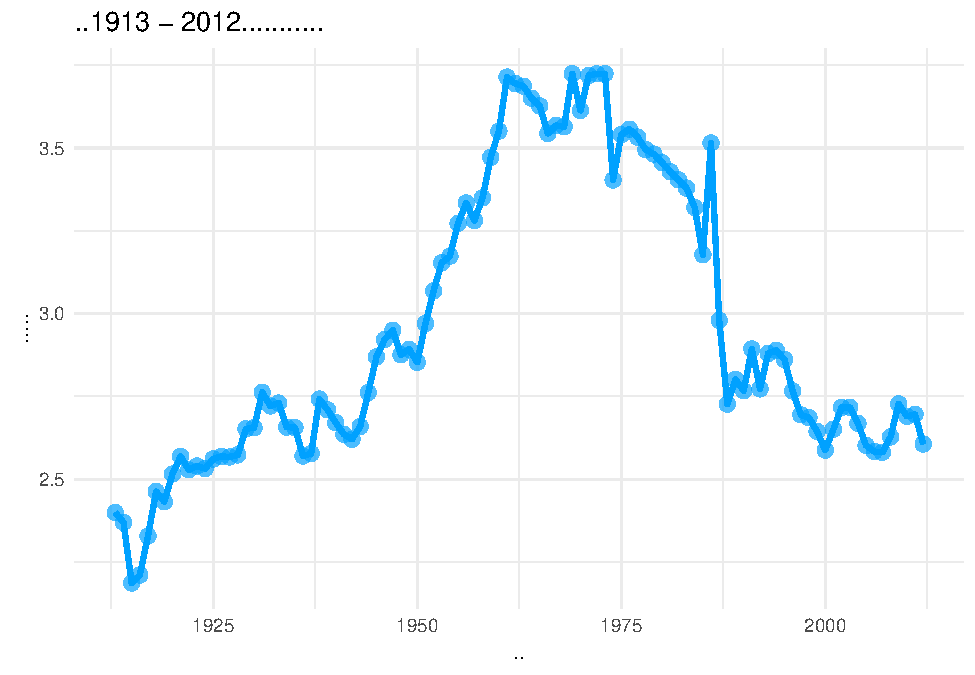
\includegraphics[keepaspectratio]{homework5_files/figure-latex/unnamed-chunk-3-1.pdf}}

\subsection{4}\label{section-2}

\begin{Shaded}
\begin{Highlighting}[]
\NormalTok{us\_data}\SpecialCharTok{$}\NormalTok{single\_ratio\_a }\OtherTok{\textless{}{-}} \DecValTok{1} \SpecialCharTok{{-}} \FunctionTok{log}\NormalTok{(}\DecValTok{10}\NormalTok{) }\SpecialCharTok{/} \FunctionTok{log}\NormalTok{(us\_data}\SpecialCharTok{$}\NormalTok{P99.income.threshold }\SpecialCharTok{/}\NormalTok{ us\_data}\SpecialCharTok{$}\NormalTok{P99.}\FloatTok{9.}\NormalTok{income.threshold)}


\ControlFlowTok{if}\NormalTok{(}\FunctionTok{any}\NormalTok{(}\FunctionTok{is.na}\NormalTok{(us\_data}\SpecialCharTok{$}\NormalTok{single\_ratio\_a))) \{}
  \FunctionTok{warning}\NormalTok{(}\StringTok{"存在NA值,可能是由于P99或P99.9为0或负值"}\NormalTok{)}
\NormalTok{  us\_data }\OtherTok{\textless{}{-}}\NormalTok{ us\_data[}\SpecialCharTok{!}\FunctionTok{is.na}\NormalTok{(us\_data}\SpecialCharTok{$}\NormalTok{single\_ratio\_a), ]}
\NormalTok{\}}




\FunctionTok{ggplot}\NormalTok{(us\_data, }\FunctionTok{aes}\NormalTok{(}\AttributeTok{x =}\NormalTok{ single\_ratio\_a, }\AttributeTok{y =}\NormalTok{ estimated\_a)) }\SpecialCharTok{+}
  \FunctionTok{geom\_point}\NormalTok{(}\AttributeTok{color =} \StringTok{"\#5ed935"}\NormalTok{, }\AttributeTok{size =} \DecValTok{3}\NormalTok{, }\AttributeTok{alpha =} \FloatTok{0.6}\NormalTok{) }\SpecialCharTok{+}
  \FunctionTok{geom\_smooth}\NormalTok{(}\AttributeTok{method =} \StringTok{"lm"}\NormalTok{, }\AttributeTok{color =} \StringTok{"gray50"}\NormalTok{, }\AttributeTok{alpha =} \FloatTok{0.2}\NormalTok{) }\SpecialCharTok{+}
  \FunctionTok{geom\_abline}\NormalTok{(}\AttributeTok{intercept =} \DecValTok{0}\NormalTok{, }\AttributeTok{slope =} \DecValTok{1}\NormalTok{, }\AttributeTok{linetype =} \StringTok{"dashed"}\NormalTok{, }\AttributeTok{color =} \StringTok{"red"}\NormalTok{) }\SpecialCharTok{+}
  \FunctionTok{labs}\NormalTok{(}
    \AttributeTok{title =} \StringTok{"单比率法 vs 多比率联合法:帕累托指数估计对比"}\NormalTok{,}
    \AttributeTok{subtitle =} \StringTok{"美国1913{-}2012年数据"}\NormalTok{,}
    \AttributeTok{x =} \StringTok{"单比率法估计的a值"}\NormalTok{,}
    \AttributeTok{y =} \StringTok{"多比率联合法估计的a值"}
\NormalTok{  ) }\SpecialCharTok{+}
  \FunctionTok{theme\_minimal}\NormalTok{()}
\end{Highlighting}
\end{Shaded}

\pandocbounded{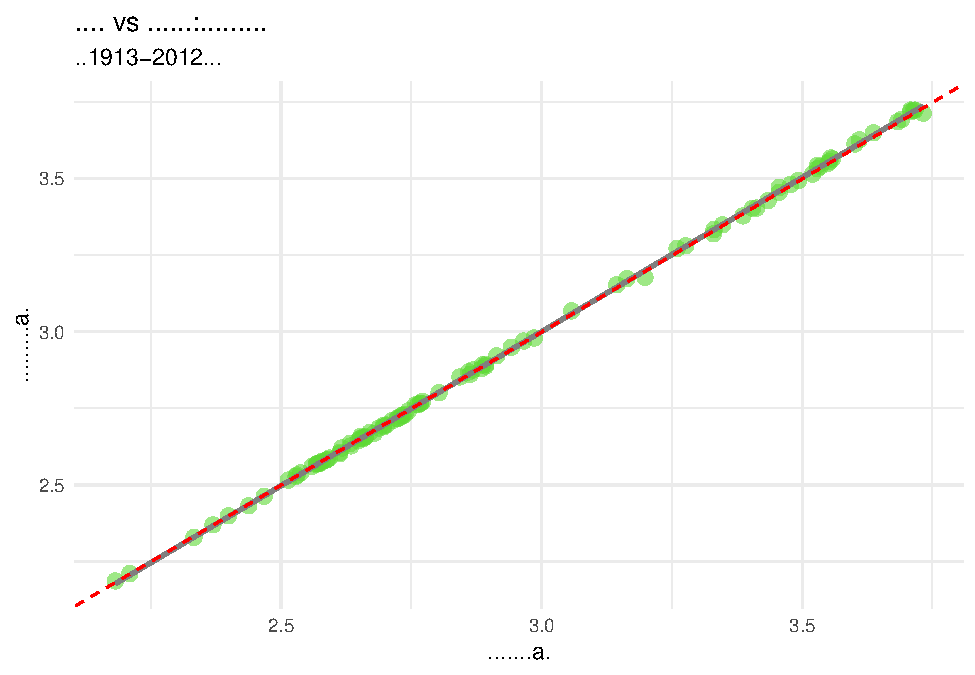
\includegraphics[keepaspectratio]{homework5_files/figure-latex/unnamed-chunk-4-1.pdf}}

\begin{Shaded}
\begin{Highlighting}[]
\NormalTok{correlation }\OtherTok{\textless{}{-}} \FunctionTok{cor}\NormalTok{(us\_data}\SpecialCharTok{$}\NormalTok{single\_ratio\_a, us\_data}\SpecialCharTok{$}\NormalTok{estimated\_a)}
\NormalTok{mean\_diff }\OtherTok{\textless{}{-}} \FunctionTok{mean}\NormalTok{(us\_data}\SpecialCharTok{$}\NormalTok{estimated\_a }\SpecialCharTok{{-}}\NormalTok{ us\_data}\SpecialCharTok{$}\NormalTok{single\_ratio\_a)}
\NormalTok{sd\_diff }\OtherTok{\textless{}{-}} \FunctionTok{sd}\NormalTok{(us\_data}\SpecialCharTok{$}\NormalTok{estimated\_a }\SpecialCharTok{{-}}\NormalTok{ us\_data}\SpecialCharTok{$}\NormalTok{single\_ratio\_a)}

\FunctionTok{cat}\NormalTok{(}\StringTok{"两种方法的相关系数:"}\NormalTok{, }\FunctionTok{round}\NormalTok{(correlation, }\DecValTok{3}\NormalTok{), }\StringTok{"}\SpecialCharTok{\textbackslash{}n}\StringTok{"}\NormalTok{)}
\end{Highlighting}
\end{Shaded}

\begin{verbatim}
## 两种方法的相关系数: 1
\end{verbatim}

\begin{Shaded}
\begin{Highlighting}[]
\FunctionTok{cat}\NormalTok{(}\StringTok{"多比率法估计平均比单比率法高:"}\NormalTok{, }\FunctionTok{round}\NormalTok{(mean\_diff, }\DecValTok{3}\NormalTok{), }\StringTok{"}\SpecialCharTok{\textbackslash{}n}\StringTok{"}\NormalTok{)}
\end{Highlighting}
\end{Shaded}

\begin{verbatim}
## 多比率法估计平均比单比率法高: 0
\end{verbatim}

\begin{Shaded}
\begin{Highlighting}[]
\FunctionTok{cat}\NormalTok{(}\StringTok{"两种方法差异的标准差:"}\NormalTok{, }\FunctionTok{round}\NormalTok{(sd\_diff, }\DecValTok{3}\NormalTok{), }\StringTok{"}\SpecialCharTok{\textbackslash{}n}\StringTok{"}\NormalTok{)}
\end{Highlighting}
\end{Shaded}

\begin{verbatim}
## 两种方法差异的标准差: 0.007
\end{verbatim}

\end{document}
